% CREATED  14 May  2015
% MODIFIED 23 July 2015
% PURPOSE present to a group of statisticians from the public health faculty at Herston

\documentclass[xcolor=svgnames,aspectratio=169]{beamer} 

\setbeamercolor{normal text}{bg=white,fg=black} 
\usecolortheme[named=blue]{structure} 
\usetheme{default} 

\usepackage{graphicx}
\usepackage{subfigure}
%\usepackage[space]{grffile}
\usepackage{rotating}
\usepackage{booktabs}
\usepackage{amsmath}
\usepackage{multicol}
\usepackage{multirow}
\usepackage{natbib}
\usepackage{bibentry}

\def\Tiny{\fontsize{1pt}{1pt}\selectfont}

\setbeamersize{text margin left=0.2em} % used to allow wide tables to fit-in a slide

\begin{document}

\title{An application of hazard function models to estimate \\ mortality rates affecting fish populations}
%\subtitle{Illustration from recent trends in the dynamic of brown tiger prawn trawl fishery in Moreton Bay}
\author{Marco Kienzle}
\institute{Qld Department of Agriculture, Fisheries - Dutton Park\\ UQ's school of Agriculture and Food Sciences - St Lucia}
\date{\today} 

%%%%%%%%%%%%%%%%%%%%%%%%%%%%%%
\frame{\titlepage}

%% %%%%%%%%%%%%%%%%%%%%%%%%%%%%%%
%% \frame{\frametitle{Fisheries stock assessment: what is it ? why we do it ?}

%% %\begin{figure}[!h]
%% %     \centering
%% %      \includegraphics[scale=0.35,angle=0]{Graphics/AtlCod.ps}
%% %    \end{figure}

%% \begin{figure}
%%    \includegraphics[width=0.275\textwidth, scale = 0.1]{Graphics/Surexploitation_morue_surpêcheEn.ps}
%%    %\hfill
%%    \includegraphics[width=0.275\textwidth, scale = 0.05, angle=-90]{Graphics/ModelOverlayedObs.ps}
%%    \vfill
%%    \includegraphics[width=0.275\textwidth, scale = 0.1]{Graphics/08COD0026.ps}
%%    %\hfill
%%    \includegraphics[width=0.275\textwidth, scale = 0.1]{Graphics/AtlCod.ps}
%% \end{figure}

%% }

%%%%%%%%%%%%%%%%%%%%%%%%%%%%%%
\frame{\frametitle{Fisheries stock assessment: what is it ? why we do it ?}

\begin{itemize}
\item governments are interested in sustainable exploitation of their natural resources
\item fishermen and research organizations collect data to assess the status of fish species
\item a mathematical model is calibrated to available data and later used to determine sustainable levels of fishing
\item Essentially, a stock assessment model estimates mortality rates (and recruitment)
\end{itemize}

\vspace{0.5cm}
Motivations for doing this work \\
\begin{itemize}
\item provide estimates of fish mortality rates using age data from a sample of catch
\item work within the likelihood framework in order to compare different models
\end{itemize}

}
%% %%%%%%%%%%%%%%%%%%%%%%%%%%%%%%
\frame{\frametitle{Age data available to fisheries scientists}

\begin{itemize}
 \item otoliths, rings\\
   \includegraphics[width=0.4\textwidth, scale = 0.5]{Graphics/08COD0026.ps}
 \item continuous time variable segmented into discrete interval (often yearly)
 \item data from a random sample of the catch
\end{itemize}

}

%%%%%%%%%%%%%%%%%%%%%%%%%%%%%%
\frame{\frametitle{Deterministic theory of fishing for a single cohort} 

%\begin{itemize}
Exponential decline a cohort through time from \cite{quin99b}
\begin{equation}
\frac{dN}{dt} = - F N - M N
\end{equation}

\begin{equation}
N(t) = N_{0} e^{-(F+M) t}
\end{equation}

%\begin{itemize}
Baranov catch equation (1910)
\begin{equation}
\frac{dC}{dt} = F N
\end{equation}

\begin{equation}
C_{0 \rightarrow \tau} = \frac{F}{M+F} N_{0} (1 - e^{-(M+F) \tau})
\end{equation}

Deterministic parameters estimations ($N_{0}, M, F$) by least square or likelihood using catches at age \\
{\color{red} PROBLEMS}: high number of parameters, convergence failure, require accurate starting values, fixing some parameters as a solution, etc...
}

%% %%%%%%%%%%%%%%%%%%%%%%%%%%%%%%
\frame{\frametitle{Survival analysis approach to a single cohort} 

Survival analysis \citep{cox84b, scimar42} using a constant hazard function

\begin{equation}
h(t; \theta) = M + F
\end{equation}

The probability density function (pdf)

\begin{equation}
f(t; \theta) = (M + F) \ e^{-(M+F)t}
\end{equation}

The likelihood \citep{edwards1992likelihood} of a sample of fish caught in the fishery ($S_{i}$) using the probability of dying in the interval $[a_{i}; a_{i+1}]$.

\begin{equation}
\mathcal{L}  = \prod_{i=1}^{n} \bigl ( \int_{t=a_{i}}^{t=a_{i+1}} f(t; \theta) \ dt \bigr ) ^ {S_{i}} 
\end{equation}

The logarithm of the likelihood was
\begin{equation}
{\rm log}(\mathcal{L}) = \sum_{i=1}^{n} S_{i} \ {\rm log} \bigl ( e^{-(M+F) \times a_{i}} - e^{-(M+F) \times a_{i+1}} \bigr )
\end{equation}

}

%%%%%%%%%%%%%%%%%%%%%%%%%%%%%%%%%
\frame{\frametitle{Can we deal with particular cases within this framework}

\begin{itemize}
\item restricted range of ages $\rightarrow$ truncated pdf
\item +group $\rightarrow$ integrate over a larger interval $ [a_{+}; \infty[ $
\end{itemize}
}

%%%%%%%%%%%%%%%%%%%%%%%%%%%%%%%%%
\frame{\frametitle{Hazard models for more complicate situations}

Fishing mortality is a function of effort (E)\\
$F(t) = q \ E(t)$ $\rightarrow h(t; \theta) = M + q \ E(t)$\\

\vspace{0.5cm}

Gear selectivity (s) varies with age\\
$F(t) = q \ s(t) \ E(t)$ $\rightarrow h(t; \theta) = M + q \ s(t) \ E(t)$\\

\begin{figure}[!h]
     \centering
      \includegraphics[scale=0.25,angle=-90]{Graphics/LogisticGearSelectivity.ps}
    \end{figure}

}

%%%%%%%%%%%%%%%%%%%%%%%%%%%%%%%%
\frame{\frametitle{Applying hazard model to data from multiple cohort}

\[
\begin{array}{cc|ccccc}
& & \multicolumn{5}{c}{ \rm{age-groups} } \\
& & 1      & \ldots & j & \ldots & n \\ \hline 
& 1 & \ldots  & & \ldots & & \ldots \\
& \vdots &  \ldots  & & \ldots & & \ldots \\
\multirow{3}{*}{\begin{sideways} years \end{sideways}} & & & & & & \\
& i & \dots  & & S_{i,j} & & \ldots \\
& \vdots &  \ldots  & & \ldots & & \ldots \\
& p & \dots  & & \ldots & & \ldots \\
\end{array}
\]

\begin{itemize}
 \item $n + p - 1$ cohorts, separability $F_{i,j} = q \ E_{i} \otimes s_{j}$
\end{itemize}

The likelihood
\begin{equation}
\mathcal{L} = \prod_{k=1}^{n+p-1} \prod_{l=1}^{r_{k}}  \bigl ( \int_{t=a_{k,l}}^{t=a_{k,l+1}} g_{k}(t; \theta) \ dt \bigr ) ^ {S_{k,l}}
\end{equation}

}

%%%%%%%%%%%%%%%%%%%%%%%%%%%%%%
\frame{\frametitle{Computer implementation of these methods}

Methods implemented in R \citep{R} in a package called Survival Analysis for Fisheries Research (SAFR) \\

\vspace{0.5cm}

Available at: \url{https://github.com/mkienzle/SurvivalAnalysisForFisheries} \\

\vspace{0.5cm}

Manuscript: \url{http://arxiv.org/abs/1501.03131}

 
}

%%%%%%%%%%%%%%%%%%%%%%%%%%%%%%
\frame{\frametitle{Testing hazard functions with Monte Carlo simulations}

Simulate a fishery using random population characteristics (recruitment, natural mortality) and random catch (catchability, effort and gear selectivity)\\

\vspace{0.5cm}

2 types of sampling to generate artificial catch data
\begin{itemize}
\item random sampling (benchmark) [strategy 1]
\item systematic [strategy 2] (weighted by catch or un-weighted)
\end{itemize}
 
}

%%%%%%%%%%%%%%%%%%%%%%%%%%%%%%
\frame{\frametitle{Hazard function models can estimate natural mortality \\when age-sample are weighted by total catch}

\begin{figure}[!h]
     \centering
      \includegraphics[scale=0.35,angle=-90]{../../Results/Graphics/Estimating-NaturalMortality4PresentationColour.ps}
    \end{figure}

}
%%%%%%%%%%%%%%%%%%%%%%%%%%%%%%
\frame{\frametitle{Sampling strategy 2 using weighted samples can estimate catchability (q)}

\begin{figure}[!h]
     \centering
      \includegraphics[scale=0.35,angle=-90]{../../Results/Graphics/Estimating-Catchability4PresentationColour.ps}
    \end{figure}

}

%%%%%%%%%%%%%%%%%%%%%%%%%%%%%%
\frame{\frametitle{Hazard function fit better than the traditional multinomial approach}

\begin{figure}[!h]
     \centering
      \includegraphics[scale=0.35,angle=-90]{../../Results/Graphics/ComparisonOfNegLL4Presentation.ps}
    \end{figure}

}

%%%%%%%%%%%%%%%%%%%%%%%%%%%%%%
\frame{\frametitle{Example of fit to real data (Qld mullet fishery)}

\begin{figure}[!h]
     \centering
      \includegraphics[scale=0.35,angle=-90]{Graphics/MulletDataOverlayedWithSurvivalAnalysisModel.ps}
    \end{figure}

}

%%%%%%%%%%%%%%%%%%%%%%%%%%%%%%
\frame{\frametitle{Conclusions}

\begin{itemize}
\item hazard functions seems perfectly suited to estimate mortality rates for fisheries research
\item likelihood ratios suggest survival analysis provides a better model of mortality rates than the traditional one
\item for the moment, survival analysis seems fairly unknown in fisheries research circles

\end{itemize}

\vspace{0.5cm}
\begin{table}
\begin{center}
\begin{tabular}{|l | c | c|}
\hline
Characteristics        & Traditional methods & Survival analysis \\
\hline \hline
likelihood based       & not always          & yes               \\
use all data           & not always          & yes               \\
estimate nat. mort.    & no                  & yes               \\
tested with MC         & not always          & yes               \\
\hline
\end{tabular}
\end{center}
\end{table} 
}

%%%%%%%%%%%%%%%%%%%%%%%%%%%%%%
\frame{\frametitle{Thank you for your attention}

\begin{itemize}
\item Any comments about applying survival analysis to estimate fish mortality rates ?
\item Do you know of any R package readily available to process fish-age data ?
\item Would you like to contribute your expertise to articles on this topic ?
\end{itemize}

\nobibliography{/home/mkienzle/mystuff/Bibliography/a-JLong,/home/mkienzle/mystuff/Bibliography/Biblio}
\bibliographystyle{plainnat}

}

\end{document}
